\documentclass[../main.tex]{subfiles}
\graphicspath{{\subfix{../Images/}}}
\begin{document}

\lhead{Еров}
\subsection{Формула Валлиса}
Сама формула: $\frac{1}{k}{(\frac{(2k)!!}{(2k-1)!!})}^{2} \underset{k \to \infty}{\longrightarrow} \pi$ \\\\
\textbf{Вывод формулы:} \\
Рассмотрим $I_n = \int\limits_{0}^{\frac{\pi}{2}}\sin{x}^{n}dx$: (пока без пруфа)\\\\
$n$ -- нечетное: $I_n = \frac{(n - 1)!!}{n!!} \frac{\pi}{2}$ \\\\
$n$ -- четное: $I_n = \frac{(n - 1)!!}{n!!}$ \\\\
При $x \in [0, \frac{\pi}{2}]$: $\sin{x}^{2k+1} \leq \sin{x}^{2k} \leq \sin{x}^{2k-1}$ \\\\
Проинтегрируем от 0 до $\frac{\pi}{2}$: \\\\
$\frac{(2k)!!}{(2k+1)!!} \leq \frac{(2k-1)!!}{(2k)!!} \frac{\pi}{2} \leq \frac{(2k-2)!!}{(2k-1)!!}$. Домножим на $\frac{(2k)!!}{(2k-1)!!}$: \\\\
${(\frac{(2k)!!}{(2k+1)!!})}^{2} \frac{1}{2k+1} \leq \frac{\pi}{2} \leq \frac{1}{2k} {(\frac{(2k)!!}{(2k+1)!!})}^{2}$. Пусть $A_k := {(\frac{(2k)!!}{(2k+1)!!})}^{2}$ \\\\
Рассмотрим разность правой и левой частей: \\\\
$A_k(\frac{1}{2k} - \frac{1}{2k-1}) = \frac{A_k}{2k(2k-1)}$, что в силу левого неравенства $\leq \frac{\pi}{4k} \underset{k \to \infty}{\longrightarrow} 0$ \\\\
Значит, длина промежутка (из неравенства), содержащего точку $\frac{\pi}{2}$ стремится к 0, и в частности, его границы стремятся к $\frac{\pi}{2}$\\\\
Запишем это для правого неравенства:\\\\
$\frac{1}{k}{(\frac{(2k)!!}{(2k-1)!!})}^{2} \underset{k \to \infty}{\longrightarrow} \pi$. Что равносильно $\sqrt{\pi} = \lim{\frac{1}{\sqrt{k}} \frac{(2k)!!}{(2k-1)!!}}$

\newpage


\lhead{Еров}
\subsection{Формула Стирлинга}
Сама формула: $n!$ $\mathtt{\sim}$  ${n}^{n} {e}^{-n} \sqrt{n} \sqrt{2\pi}$ \\\\
\textbf{Вывод формулы:} \\\\
Рассмотрим $f(x) = \ln{x}$ \\\\
По формуле Эйлера-Маклорена:\\\\
$\sum\limits_{i=1}^{n} {\ln{i}} = \int\limits_{1}^{n} {\ln{x}dx} + \frac{\ln{n}}{2} - \frac{1}{2} \int\limits_{1}^{n} {\frac{1}{{x}^{2}} \{x\}(1-\{x\})dx}$, последнее слагаемое возрастает как функция от $n$ и ограничено, тогда верно: \\\\
$\sum\limits_{i=1}^{n} {\ln{i}} = n\ln{n} - n + \frac{\ln{n}}{2} + c_1 + o(1)$. Перейдем к экспоненте: \\\\
$n! = {n}^{n} {e}^{-n} \sqrt{n}\cdot c \cdot {e}^{o(1)}$, где $c := {e}^{c_1}$ \\\\
Заметим, что ${e}^{o(1)} \rightarrow 1$, поэтому тут верна эквивалентность $n!$ $\mathtt{\sim}$  ${n}^{n} {e}^{-n} \sqrt{n} \cdot c$, осталось найти $c$. \\\\
Возьмем формулу Валлиса и чуток распишем ее: \\\\
$\sqrt{\pi} = \lim{\frac{1}{\sqrt{k}} \frac{(2k)!!}{(2k - 1)!!}} = \lim{\frac{1}{\sqrt{k}} \frac{{2}^{k}\cdot{k!}}{(2k - 1)!!}}$ (домножим на $(2k)!!$):\\\\
$\sqrt{\pi} = \lim{\frac{1}{\sqrt{k}} \frac{{2}^{2k}\cdot {(k!)}^{2}}{(2k)!}}$ (заменяем факториалы на эквивалентные по полученной формуле с константой): \\\\
$\sqrt{\pi} = \lim{\frac{1}{\sqrt{k}} \frac{{2}^{2k}\cdot{c}^{2}\cdot{k}^{2k}\cdot k}{c\cdot{(2k)^{2k}\cdot{e}^{-2k}\cdot\sqrt{2k}}}} = \lim{\frac{c}{2}}$
$\Rightarrow c = \sqrt{2\pi}$\\\\
$\Rightarrow n!$ $\mathtt{\sim}$  ${n}^{n} {e}^{-n} \sqrt{n} \sqrt{2\pi}$
\newpage


\lhead{Григоренко}
\subsection{Неравенство Йенсена для сумм}
$f$~--- выпуклая на $\left<a,b\right>$. Тогда
\begin{equation*}
    \forall x_1,\dots,x_n \in \left<a,b\right> \quad
    \forall \alpha_1,\dots,\alpha_n \quad
    \left(\alpha_i\ge0\right)\land\left(\sum_{i=1}^{n}\alpha_i=1\right) \Rightarrow
    f\left(\sum_{i=1}^{n}\alpha_i x_i\right)\le\sum_{i=1}^{n}\alpha_i f(x_i)
\end{equation*}
\begin{proof}
    Для $x_1=x_2=\dots=x_n$ тривиально.
\begin{gather*}
    \text{Покажем, что }\sum\limits_{i=1}^{n}\alpha_i x_i\overset{\text{def}}{=}x^*\in\left<a,b\right>\\
    \min_i x_i \le x^* \le \left(\sum_{i=1}^{n}\alpha_i\right)\max_i x_i = \max_i x_i 
\end{gather*}
В $x^*$ можно провести опорную прямую $y=kx+b$
\begin{equation*}
    f(x^*)=kx^*+b=
    k\left(\sum_{i=1}^{n}\alpha_i x_i\right)+b=
    \sum_{i=1}^{n}k\alpha_i x_i+\sum_{i=1}^{n}\alpha_i b=
    \sum_{i=1}^{n}\alpha_i (k x_i+b)\le
    \sum_{i=1}^{n}\alpha_i f(x_i)
\end{equation*}
\end{proof}
\newpage


\lhead{Григоренко}
\subsection{Неравенство Йенсена для интегралов. }
\begin{equation*}
    \begin{cases}
        f\text{~--- выпуклая на }\left<A,B\right>\\
        \varphi:[a,b]\to\left<A,B\right>\text{~--- непрерывная}\\
        \lambda:[a,b]\to\left<A,B\right>\text{~--- (кусочно-)непрерывная}\\
        \int_a^b\lambda(t)dt=1
    \end{cases}
    \Rightarrow
    f\left(\int_a^b \lambda(t)\varphi(t)dt\right)\le
    \int_a^b \lambda(t)f(\varphi(t))dt
\end{equation*}
\begin{proof}
\begin{gather*}
    m\overset{\text{def}}{=}\inf \varphi \\
    M\overset{\text{def}}{=}\sup \varphi \\
    m =
    m \int_a^b\lambda(t)dt \le
    \int_a^b\lambda(t)\varphi(t)dt \le
    M\int_a^b\lambda(t)dt = M \\
    x^* \overset{\text{def}}{=} \int_a^b\lambda(t)\varphi(t)dt \Rightarrow x^*\in\left<A,B\right>
\end{gather*}

Для $M=m$ тривиально.

$y=kx+c$ опорная прямая в точке $x^*$ графика $f$.
\begin{equation*}
    f(x^*)=kx^*+c=k\int_a^b\lambda\varphi+c\int_a^b\lambda=
    \int_a^b (k\varphi+c)\lambda \le
    \int_a^b f(\varphi(t))\lambda(t)dt
\end{equation*}
\end{proof}
\newpage


\lhead{M3137-y2019}
\subsection{Неравенство Коши (для сумм и для интегралов)}
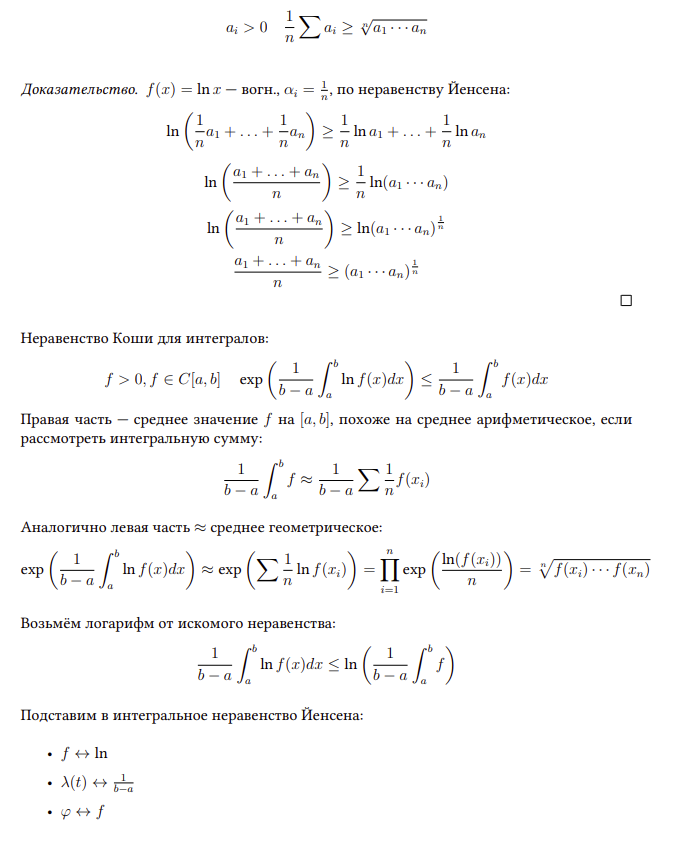
\includegraphics[scale = 1]{Images/2.37.png}
\newpage


\end{document}